\section{Introduction}\label{sec:intro}

Text-to-SQL systems translate natural-language questions into executable SQL queries over relational databases and let users retrieve structured records without writing query code~\cite{yu2018spider,li2023bird}. In-context prompting of proprietary large language models (LLMs) is widely adopted for the task~\cite{pourreza2023dinsql,gao2024dailsql}, but calling their application programming interfaces (APIs) sends questions and schemas to a third-party provider, with risks for data privacy and recurring inference costs, which fine-tuning an open model for deployment on local machines avoids~\cite{li2024codes}. Small language models (SLMs) of \setting{models.size.min} to \setting{model.size} parameters offer fast inference and suit deployment at the edge~\cite{sheng2025slmsql}, so that an organization can fine-tune one and serve it on its own hardware.

A single organization, however, typically holds few databases and annotated question-SQL pairs, and data isolation precludes pooling schemas, records or annotations across organizations. Federated learning~\cite{mcmahan2017fedavg} lets several organizations train one shared SLM while their data remain on their premises, and only the trained model is deployed. We use \textit{federated Text-to-SQL} for the federated training of a shared Text-to-SQL model across clients, following Zhang et al.~\cite{zhang2023fl4sp}. To limit the computation and communication of the clients, federated frameworks for LLMs train a low-rank adaptation (LoRA) adapter~\cite{hu2022lora} under federated averaging with supervised fine-tuning (FedAvg SFT)~\cite{mcmahan2017fedavg,ye2024openfedllm}.

Neither federated SFT nor federated preference optimization as published executes a query of the model on the databases of the clients. FedAvg SFT~\cite{mcmahan2017fedavg,ye2024openfedllm,zhang2023fl4sp} trains each client on the one gold SQL query of each question with a token-averaged negative log-likelihood (NLL) loss (Section~\ref{sec:formulation}). The model generates no query during training, and neither the gold SQL query nor a query of the model is executed, so no execution result enters the loss. OpenFedLLM~\cite{ye2024openfedllm} brings direct preference optimization (DPO)~\cite{rafailov2023dpo} to federated learning as federated DPO (FedDPO), on helpfulness and harmlessness. In FedDPO, each client keeps one preference dataset, the reference model is fixed through the federated process, and the loss is DPO alone, so that training never uses the queries of the current global model. Centralized methods for Text-to-SQL use execution feedback through preference optimization or reinforcement learning on data held in one place~\cite{tao2024codelutra,zhai2025excot,papicchio2025think2sql,yao2026arctic}, whereas in federated learning only the client holds its databases.

\begin{figure}[!t]
\centering
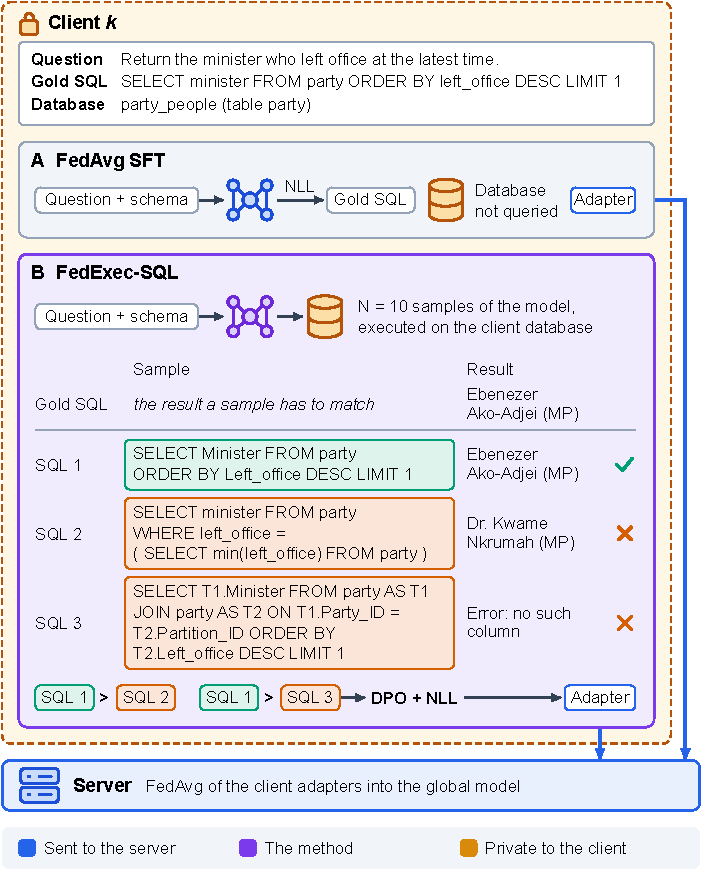
\includegraphics{figures/fig_idea.pdf}
\caption{Local supervision on one BIRD training question (database \texttt{language\_corpus}) within the dashed boundary of client~$k$. \panel{a}~In federated averaging with supervised fine-tuning (FedAvg SFT), the prompt (schema, question, and evidence) and gold SQL query define the negative log-likelihood (NLL) loss, and the database is not queried. \panel{b}~In the first preference round of \method{} (from the global model after \setting{rounds.warmup} warm-up rounds, temperature~\setting{pref.t}, at most \setting{pref.tokens} new tokens), executing $N = {}$\setting{pref.samples} samples on \texttt{language\_corpus} yields eight correct samples, one incorrect result, and one execution error. The table displays the samples of the $M = {}$\setting{pref.pairs} preference pairs built for this question beside the gold execution result, where two distinct correct samples with identical SQL text (first row) are paired against the incorrect result and the execution error (second and third rows) under the direct preference optimization (DPO) plus NLL loss.}
\label{fig:idea}
\end{figure}

Executing queries sampled from the model on the client's database and comparing their results with that of the gold SQL query turns the one gold SQL query of a question into several labeled queries of the model's own, correct and incorrect (Fig.~\ref{fig:idea}, Section~\ref{sec:supervision}). Only the client can produce these labels, since only the client holds the database.

We propose \method, a federated learning framework for Text-to-SQL that trains on this execution-derived supervision. It has four components (Section~\ref{sec:overview}, Fig.~\ref{fig:overview}). \textit{Supervised warm-up} runs the first rounds as rounds of FedAvg SFT on the gold SQL queries, so that fewer training questions have only incorrect samples. In each of the following preference rounds, \textit{client-side execution labeling} samples several queries per question from the current global model and labels each by executing it on the client's database against the result of the gold SQL query. \textit{On-policy pair construction} forms preference pairs of a correct and an incorrect sample from these labels. The \textit{preference objective} trains the adapter with a DPO term, whose reference model is the current global model, plus an NLL term on the correct sample of each pair, and the server averages the adapters by the pair counts of the clients. A preference round thus renews the pairs and the reference model together. In every round, a client sends the same adapter as in FedAvg SFT, and a preference round adds client computation for sampling, labeling and training.

We evaluate \method{} with the SLM \setting{model} (\setting{model.size} parameters)~\cite{hui2024qwen25coder} on BIRD~\cite{li2023bird} and Spider~\cite{yu2018spider}, with \fact{split.bird.a0.1.k5.clients} clients that all take part in every round and hold disjoint sets of databases (Section~\ref{sec:fed-setups}). At \setting{rounds.total} rounds, \method{} reaches \ex{bird}{k2}{4}\% execution accuracy (EX) on BIRD dev against \ex{bird}{fedavg}{4}\% for FedAvg SFT, a gain of \gap{bird}{fedavg}{4}{k2}{4} points, and \ex{spider}{k2}{4}\% on Spider test against \ex{spider}{fedavg}{4}\%, a gain of \gap{spider}{fedavg}{4}{k2}{4} points. Further rounds of FedAvg SFT do not close the gap: its highest EX on BIRD dev, \ex{bird}{fedavg}{3}\% after the third round, is \gap{bird}{fedavg}{3}{k2}{4} points below \method. On BIRD dev, \method{} is also above FedDPO run on the first execution-labeled pairs of \method, with the pairs and the reference model of that round fixed and the DPO loss alone, by \gap{bird}{feddpo}{4}{k2}{4} EX points and \tsgap{bird}{feddpo}{4}{k2}{4} points of test-suite accuracy (TS). Against FedAvg SFT, execution errors fall by about half on both benchmarks, from \nerr{bird}{fedavg}{4} to \nerr{bird}{k2}{4} on BIRD dev, while incorrect results do not fall. With the settings of the preference rounds held equal, \method{} is \gap{bird}{k2}{4}{rft}{4} EX points above the variant trained without the preference term on BIRD dev (Section~\ref{sec:ablation}). Each difference named in this paragraph is significant under the test of Section~\ref{sec:stat-test}.

In summary, we make four contributions:
\begin{itemize}
\item We identify the databases of the clients as a source of execution-derived supervision that federated fine-tuning leaves unused, and introduce, to our knowledge, the first federated training method for Text-to-SQL that uses it (Sections~\ref{sec:rel-fedsql} and~\ref{sec:supervision}).
\item We design \method{} with supervised warm-up, client-side execution labeling, on-policy pair construction and a preference objective of a DPO term and an NLL term (Section~\ref{sec:method}). Each preference round renews the pairs and the reference model together, and only the LoRA adapter and its integer weight leave a client.
\item We show that, at the same number of rounds, \method{} is above FedAvg SFT on BIRD dev and Spider test with about half as many execution errors, and that on BIRD dev it is above FedDPO run on the first execution-labeled pairs of \method under EX and TS (Sections~\ref{sec:main} and~\ref{sec:analysis}). We measure what each component adds and what a client pays in computation (Sections~\ref{sec:ablation} and~\ref{sec:cost}).
\item We release our code, federated client splits, and evaluation predictions for every row of the tables.
\end{itemize}
